\chapter{Validations}
\label{c:vali}

\section{Figure Example}
\label{s:figure}

Figure~\ref{f:media-score-cons} shows party affiliations of users on media fan pages against our estimate. 

\begin{figure}
\begin{center}
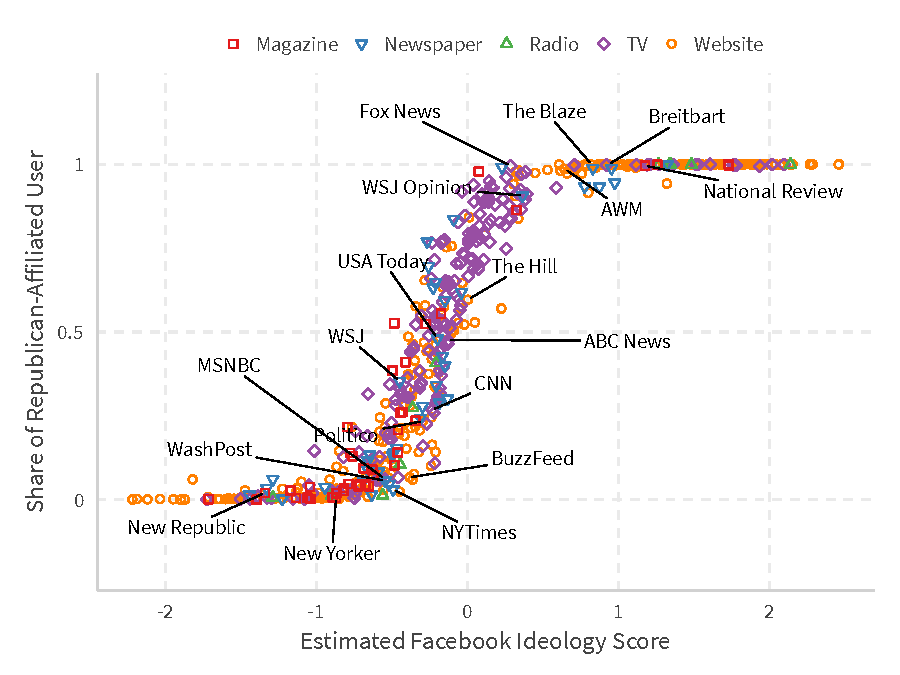
\includegraphics[width=\textwidth]{media-score-cons.pdf}
\caption{Validation of Media Slant}
\label{f:media-score-cons}
\floatfoot{{\it Notes}: 
A user is {\it Republican-affiliated} if their likes in all politicians are more for Republicans.
We only count user once a day on a page if they like more than one post on that day on that page.
We then sum all this kind of daily users up across each day.
Data ranges from 2015-01-01 to 2017-03-31.
}
\end{center}
\end{figure}
